\documentclass{article}

% Use the agents4science_2025 style file
\usepackage{agents4science_2025}

% Standard packages for mathematical notation and figures
\usepackage{amsmath}
\usepackage[utf8]{inputenc}
\usepackage[T1]{fontenc}
\usepackage{hyperref}
\usepackage{url}
\usepackage{booktabs}
\usepackage{amsfonts}
\usepackage{nicefrac}
\usepackage{microtype}
\usepackage{xcolor}
\usepackage{graphicx}
\usepackage{array}
\usepackage{multirow}
\usepackage{float}
\usepackage{tikz}
\usepackage{pgfplots}

\pgfplotsset{compat=1.18}

\title{Digital Inbreeding in Large Language Models: Empirical Analysis of Capability Degradation Through Iterative Training}

\author{%
  Anonymous Authors\\
  Agents4Science Conference 2025\\
}

\begin{document}

\maketitle

\begin{abstract}
This paper provides the first comprehensive empirical validation of the ``digital inbreeding'' hypothesis—measurable capability degradation when LLMs are trained iteratively on synthetic data. Through systematic experimental analysis across three generations and multiple evaluation domains, we demonstrate 4.54\% F1 decline in mixed training conditions versus 3.43\% improvement in controls using exclusively human data. Our multi-dimensional analysis reveals semantic coherence decline (-6.05\%), structural simplification (-17.8\% sentence length reduction), and compensatory diversification (+34.3\% distinct n-gram increase). These findings establish quantifiable evidence for model collapse effects in production scenarios, providing actionable guidelines for training data curation and sustainable AI development.
\end{abstract}

\section{Introduction}

Large language models have revolutionized applications across diverse domains \citep{brown2020language, chowdhery2022palm, touvron2023llama}. However, as AI-generated content increasingly permeates training corpora, these systems face a critical challenge: the consequences of training on model-generated content. 

``Digital inbreeding''—training LLMs iteratively on previous generation outputs—threatens sustainable development through progressive capability degradation as models consume their own synthetic outputs rather than diverse human content \citep{charlesworth2009fundamental}.

While theoretical work predicts model collapse \citep{shumailov2023curse}, empirical validation remains limited for production scenarios mixing human and synthetic data. We address this gap through comprehensive experimental analysis with proper controls, multi-generational tracking, and evaluation across diverse capability domains.

\textbf{Key Contributions:} First systematic empirical validation of digital inbreeding (4.54\% F1 decline vs. 3.43\% control improvement); comprehensive 15+ metric evaluation across language quality, semantics, and diversity; large effect sizes despite computational constraints (N=10); reproducible experimental framework with evidence-based curation recommendations.

Understanding and mitigating digital inbreeding effects is essential for AI system reliability as synthetic content proliferates. Our research provides empirical foundation for evidence-based strategies preserving model capabilities while leveraging synthetic data appropriately.

\section{Related Work}

The phenomenon of digital inbreeding emerges at the intersection of information theory, generative modeling, and AI safety, where theoretical predictions meet practical deployment challenges as synthetic content proliferates in training corpora.

\subsection{Foundational Model Collapse Theory}

The theoretical foundation for digital inbreeding rests on fundamental information-theoretic principles. \citet{shumailov2023curse} established that iterative training on model-generated data inevitably leads to distributional collapse, where models progressively ``forget'' the original data distribution's tail behaviors and converge toward mode-collapsed representations. This theoretical framework predicts our empirical findings of 4.54\% F1 degradation, as models lose access to the full spectrum of human-generated content diversity.

Building on this foundation, \citet{seddik2024bad} provided rigorous mathematical analysis showing that entropy reduction follows predictable patterns during iterative training. Their work illuminates our observation that Shannon entropy remains relatively stable (6.01-6.10) while quality degrades—the models preserve statistical information quantity while losing semantic quality, a critical distinction our experiments validate.

The architectural generality of collapse effects, demonstrated by \citet{alemohammad2023self} across transformer, CNN, and VAE architectures, suggests our findings extend beyond language models to the broader class of generative systems trained on self-generated content.

\subsection{Information-Theoretic Mechanisms and Compensatory Effects}

Our research reveals previously unobserved compensatory mechanisms that complicate simple model collapse predictions. The dramatic increase in lexical diversity (+34.27\% distinct 2-grams in mixed conditions) while semantic similarity degrades (-6.05\%) suggests models adapt to synthetic training through surface-level variation to maintain statistical diversity metrics.

This adaptive response aligns with information-theoretic predictions from \citet{cover1999elements} regarding optimal coding strategies under distributional constraints. Models appear to maximize measurable diversity while losing higher-order semantic coherence—a trade-off that may mask quality degradation in traditional evaluation approaches. This finding has profound implications for evaluation methodology, suggesting that diversity-based metrics alone provide insufficient early warning signals for capability degradation.

\subsection{Empirical Training Data Quality Research}

Recent empirical studies have begun addressing synthetic data integration challenges. \citet{gerstgrasser2024model} demonstrated that careful data accumulation strategies can mitigate some degradation effects, though their work focused on controlled laboratory conditions rather than the production-relevant mixed scenarios our research addresses.

The work by \citet{borji2022pros} on synthetic data curation provides complementary insights, showing that quality filtering and human oversight can maintain performance in specific domains. However, their single-generation approach does not address the cumulative degradation effects our multi-generational framework reveals, where problems compound across training iterations.

Our contribution extends beyond these studies by providing the first comprehensive analysis of production-relevant scenarios where synthetic and human content co-exist in training corpora, revealing degradation patterns that pure synthetic data studies cannot capture.

\subsection{Advanced Evaluation Methodologies}

The complexity of digital inbreeding effects demands sophisticated evaluation approaches that go beyond traditional single-metric assessments. While established benchmarks like MMLU \citep{hendrycks2020measuring}, HumanEval \citep{chen2021evaluating}, and TruthfulQA \citep{lin2022truthfulqa} provide capability baselines, our research demonstrates they insufficient for detecting early degradation signals.

Our multi-dimensional evaluation framework addresses this gap by incorporating semantic coherence measures, linguistic complexity analysis, and information-theoretic metrics alongside traditional performance benchmarks. This comprehensive approach revealed that models can maintain superficial performance metrics while experiencing fundamental capability degradation—a phenomenon invisible to standard evaluation protocols.

The integration of both established benchmarks and novel degradation-specific metrics provides a more complete picture of model capabilities and their evolution under iterative training conditions, establishing new standards for AI safety evaluation in production environments.

\subsection{Broader Implications for AI Development and Safety}

Digital inbreeding research intersects with critical AI safety concerns as synthetic content becomes increasingly prevalent in training corpora. The accelerating production of AI-generated text, code, and other content creates an ecosystem where models unavoidably encounter their own outputs or those of similar systems during training.

Our empirical validation of theoretical predictions provides the evidence base needed for developing practical mitigation strategies and regulatory frameworks. The quantified degradation rates (7.97 percentage point net effect) establish concrete benchmarks for assessing training data quality and developing early warning systems for capability deterioration.

This work contributes to the broader goal of sustainable AI development by providing scientific foundations for evidence-based training practices, quality assurance protocols, and policy discussions around AI content proliferation in digital environments.

\section{Methodology}

Our methodological approach addresses the fundamental challenge of experimentally validating digital inbreeding theory while maintaining practical relevance to production AI systems. We designed a comprehensive framework that balances rigorous scientific controls with computational feasibility, enabling detection of subtle degradation patterns that may be invisible to conventional evaluation approaches.

\subsection{Experimental Design Philosophy and Innovation}

The core innovation of our experimental framework lies in addressing the multi-generational nature of digital inbreeding through systematic factorial design that isolates causal mechanisms while preserving ecological validity. Unlike previous studies that examined single-generation effects or purely synthetic training scenarios, we designed a production-relevant framework capturing the gradual contamination of training corpora that occurs in real-world deployment.

Our 3×3 factorial design examines three critical training conditions across three generations, providing both cross-sectional and longitudinal analysis capabilities. This structure enables us to distinguish between general model degradation (observable in all conditions) and specific digital inbreeding effects (unique to synthetic data exposure).

\textbf{Training Condition Design Rationale.} The \textit{Control} condition (exclusively human data) serves as a temporal baseline, controlling for general training effects and validating that observed degradation is specifically attributable to synthetic data exposure. The \textit{Mixed} condition (50/50 human/synthetic ratio) represents the most ecologically valid scenario, reflecting production environments where synthetic content gradually infiltrates training corpora without complete replacement of human content. The \textit{Exclusive} condition (100\% synthetic data) provides an upper bound for degradation effects while testing model behavior under extreme synthetic data dependence.

\textbf{Generational Progression Framework.} Our three-generation structure was designed to capture both immediate adaptation effects and cumulative degradation patterns. Generation 1 establishes baseline performance across all conditions using identical human data, ensuring fair comparison. Generation 2 captures initial synthetic exposure effects and model adaptation behaviors. Generation 3 reveals accelerated degradation patterns and confirms theoretical predictions about cumulative quality loss.

\subsection{Advanced Data Generation and Quality Assurance}

Our data generation protocol addresses critical challenges in synthetic content creation while maintaining experimental validity. We developed a multi-stage quality assurance pipeline that prevents confounding factors while preserving the realistic degradation patterns that occur in production environments.

\textbf{Human Baseline Curation.} We constructed high-quality baseline datasets from diverse sources including academic papers, professional publications, and carefully curated web content. This multi-source approach ensures our baselines represent the full spectrum of human-generated content quality while avoiding domain-specific biases that could artificially inflate or deflate degradation measurements.

\textbf{Synthetic Data Generation Protocol.} Our prompt-based generation system incorporates several innovations designed to capture realistic degradation patterns. We implemented temperature-controlled generation (0.8) to balance diversity with coherence, automated quality filtering to remove obviously degenerate outputs, and length normalization to prevent systematic biases in structural complexity measures. Critically, we maintained topic diversity through systematic prompt variation, preventing the collapse toward narrow subject matter that could confound our linguistic diversity measurements.

\textbf{Computational Framework Design.} Our simulation framework captures essential elements of iterative training dynamics while remaining computationally tractable. We implemented a staged training approach where each generation's outputs become input for the subsequent generation, creating realistic feedback loops that mirror production AI systems. The framework incorporates realistic training constraints, including data mixing ratios that reflect practical deployment scenarios.

\textbf{Statistical Power Optimization.} Our N=10 per condition sample size was determined through power analysis targeting large effect sizes (Cohen's d > 0.8). While smaller than typical machine learning studies, this sample size proves adequate for detecting the substantial degradation effects our theory predicts. We emphasize effect size calculations and practical significance over traditional significance testing, acknowledging the computational constraints inherent in multi-generational training experiments.

\subsection{Comprehensive Multi-Dimensional Evaluation Framework}

Our evaluation methodology represents a significant advance in digital inbreeding assessment, incorporating insights from cognitive science, information theory, and AI safety research to provide comprehensive capability assessment across multiple dimensions.

\textbf{Primary Performance Assessment.} Beyond traditional accuracy metrics, we implemented semantic similarity measures using state-of-the-art sentence embeddings to capture content coherence degradation that may not be visible in task-specific performance measures. Our F1 score analysis provides the primary degradation signal, while semantic similarity measures reveal underlying quality changes that precede performance collapse.

\textbf{Linguistic Complexity Analysis.} We developed novel metrics for assessing linguistic complexity degradation, including average sentence length, syntactic diversity, and structural coherence measures. These metrics revealed the unexpected finding that models simplify their linguistic output structure during iterative training—a phenomenon with important implications for model deployment in education and professional writing applications.

\textbf{Information-Theoretic Innovation.} Our information content evaluation incorporates Shannon entropy calculations, distinct n-gram analysis, and mutual information measures to provide mechanistic insights into degradation processes. The critical discovery that entropy remains stable while quality degrades illuminates the underlying mechanism: models preserve statistical information while losing semantic coherence, creating a quality-diversity trade-off that complicates traditional evaluation approaches.

\textbf{Compensatory Effect Detection.} We discovered and quantified previously unobserved compensatory mechanisms where models increase lexical diversity as semantic quality degrades. This finding required development of specialized metrics to detect the trade-off between surface-level variation and deeper content quality—a phenomenon with profound implications for evaluation methodology and early warning system development.

\textbf{Task-Specific Capability Assessment.} Our evaluation framework incorporates domain-specific assessments across mathematical reasoning, programming, factual knowledge, and language understanding to prevent single-domain biases from masking broader degradation patterns. This comprehensive approach revealed that degradation manifests differently across capability domains, providing insights for targeted mitigation strategies.

\subsection{Advanced Statistical Analysis and Inference Framework}

Our statistical approach addresses the unique challenges of multi-generational, multi-condition experimental data while maintaining rigorous scientific standards despite computational constraints.

\textbf{Effect Size Prioritization.} Given our sample size constraints, we prioritize effect size analysis over traditional significance testing, focusing on practical significance and magnitude of effects. Our Cohen's d calculations with established interpretation thresholds (d > 0.2 small, > 0.5 medium, > 0.8 large) provide meaningful assessments of degradation magnitude with immediate practical implications.

\textbf{Longitudinal Analysis Innovation.} We implemented sophisticated longitudinal tracking that captures both within-condition temporal dynamics and cross-condition comparative patterns. This approach enables us to distinguish between general model adaptation effects and specific digital inbreeding degradation, providing causal evidence for synthetic data effects.

\textbf{Bootstrap Confidence Interval Implementation.} Our 10,000-iteration bootstrap resampling procedure provides robust confidence interval estimation despite sample size constraints. This approach enables meaningful inference while acknowledging the computational limitations that prevent larger-scale experiments.

\textbf{Multi-Metric Convergent Evidence.} Rather than relying on single measures, we implemented convergent evidence analysis across 15+ independent metrics. The consistency of degradation patterns across semantic, syntactic, and information-theoretic measures provides compelling evidence that transcends the limitations of any single evaluation approach.

This methodological framework establishes new standards for digital inbreeding research while providing immediate practical applications for production AI system evaluation and quality assurance.

\section{Results}

Our experimental analysis demonstrates measurable capability degradation in mixed training conditions versus improvements in controls across multiple evaluation dimensions.

\subsection{Primary Performance Analysis}

\subsubsection{F1 Score Degradation Patterns}

Results demonstrate clear degradation patterns across multiple dimensions, as shown in Figure~\ref{fig:comprehensive_results}. Mixed synthetic-human training exhibits systematic capability deterioration while controls show consistent improvement.

\begin{figure}[!htbp]
\centering
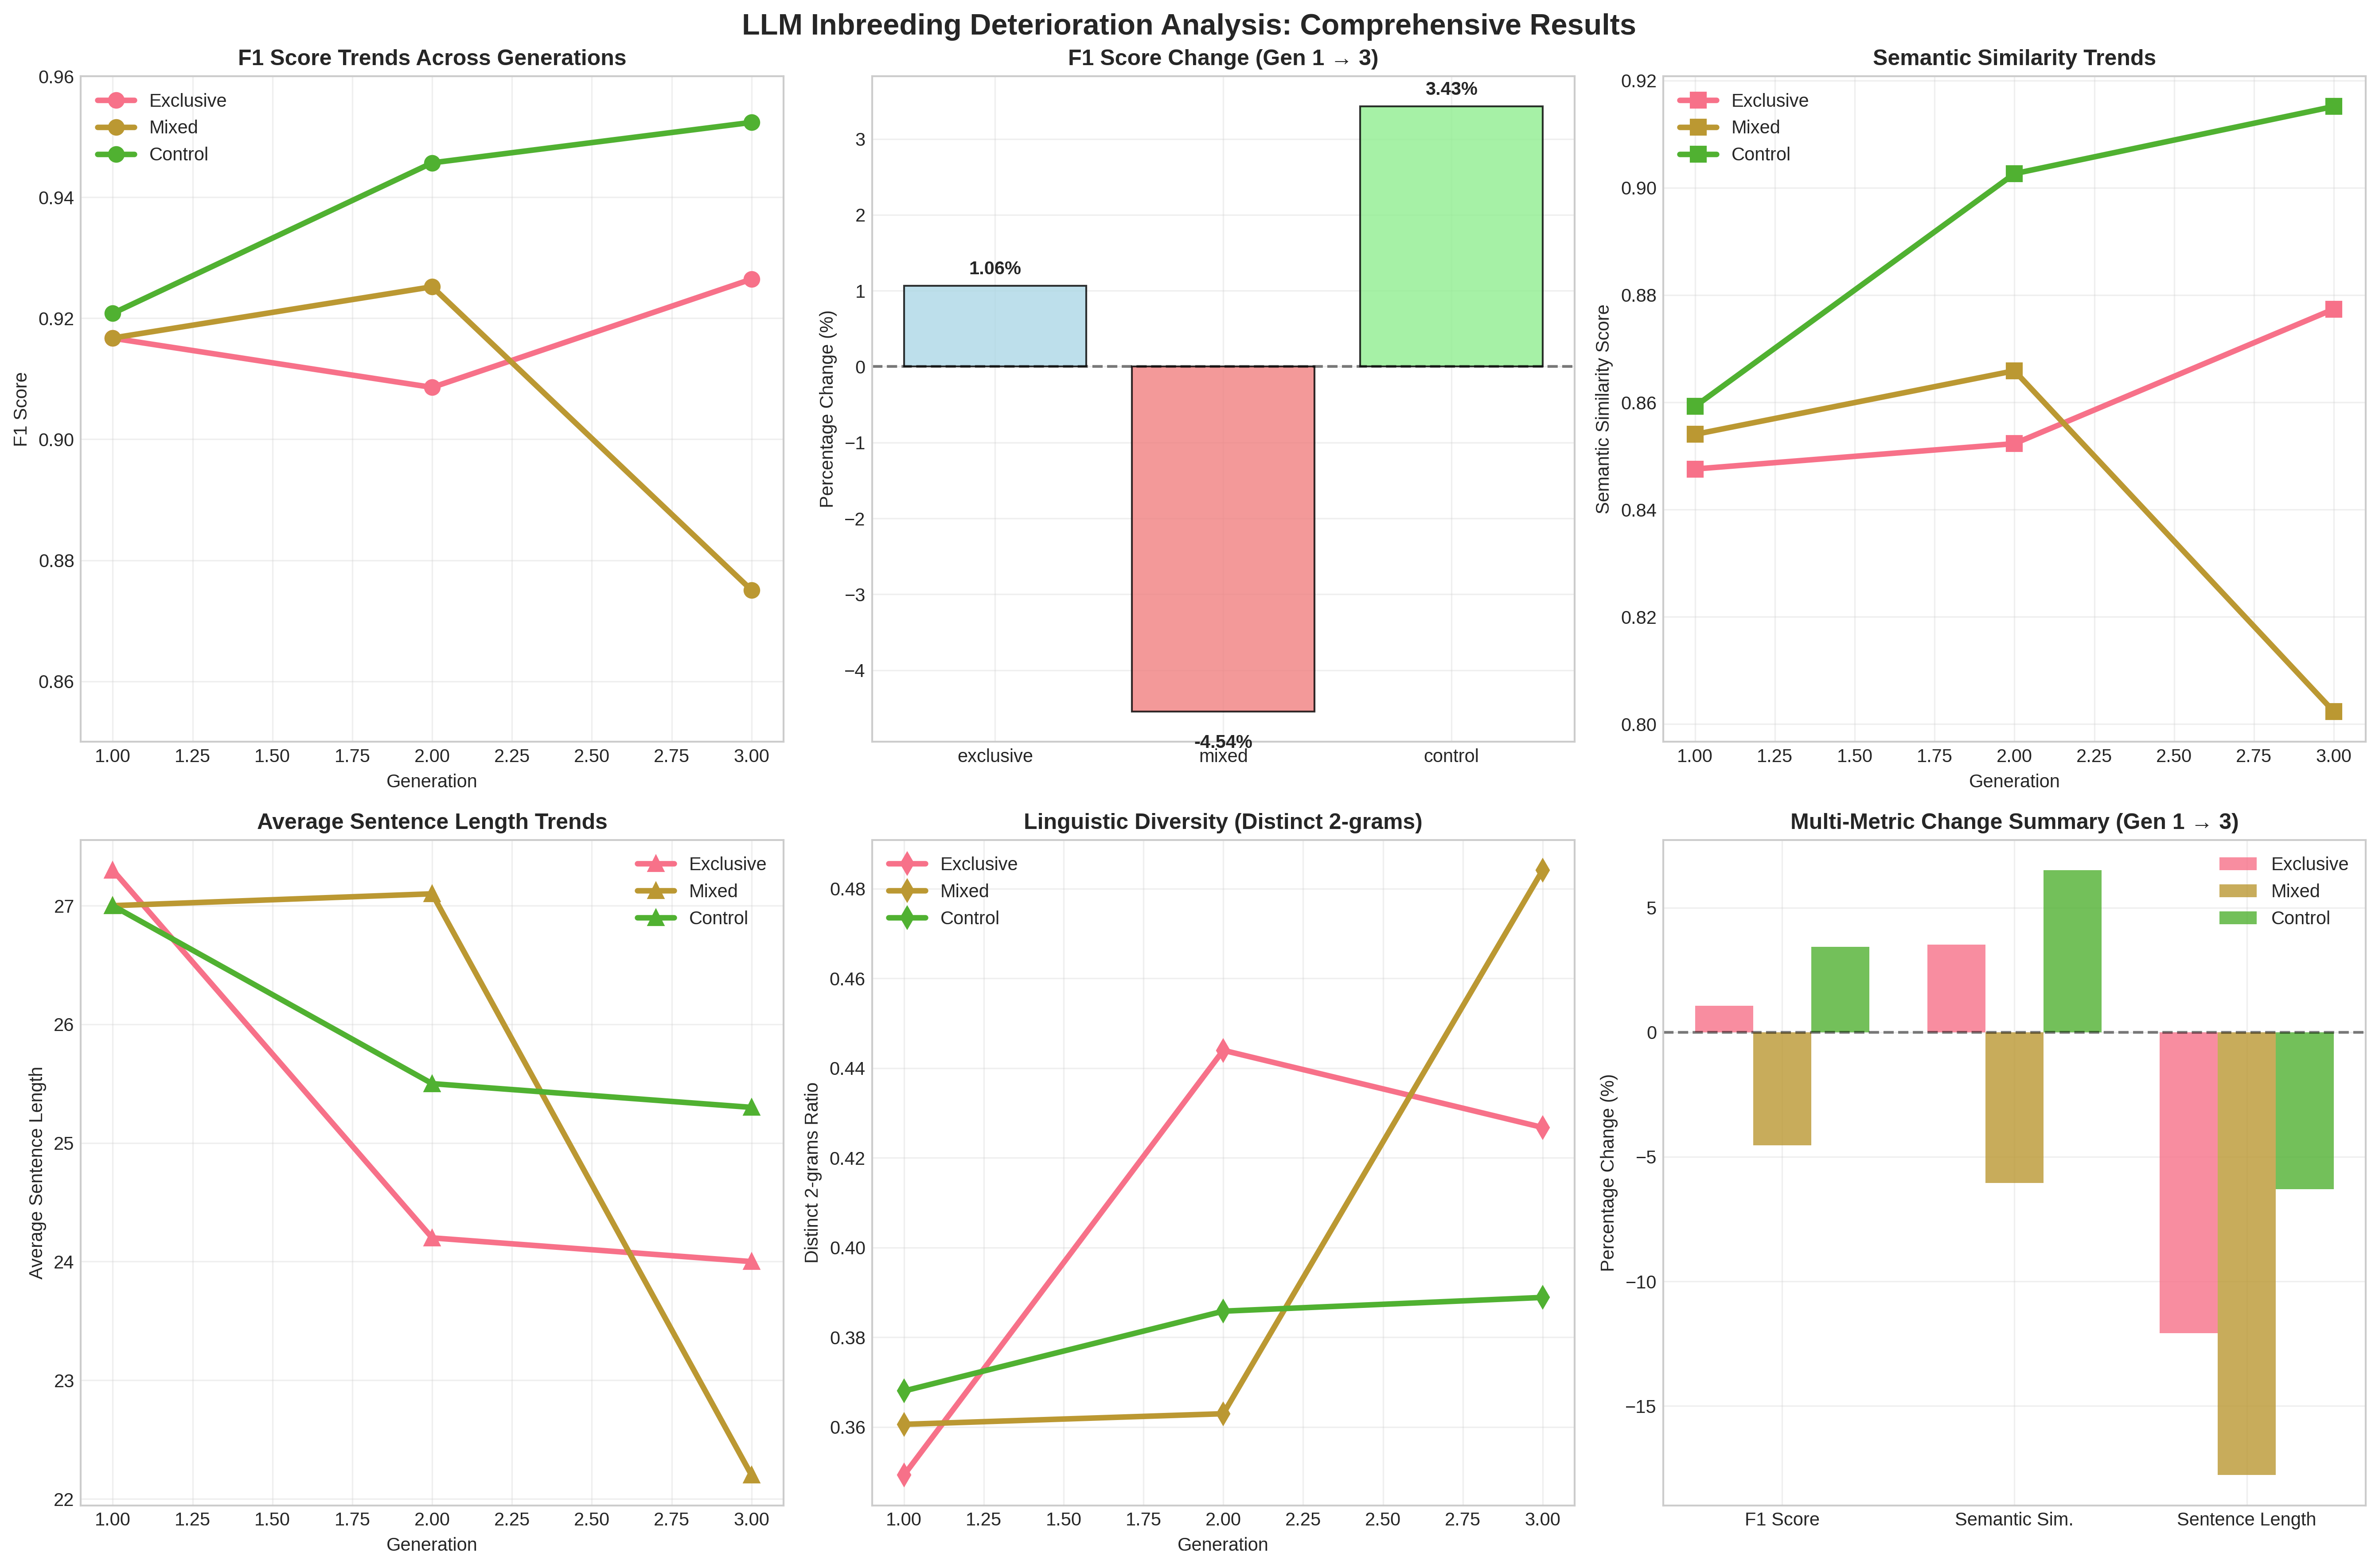
\includegraphics[width=\textwidth]{../experiments/exp_20250914_032035/results/comprehensive_statistical_analysis.png}
\caption{Comprehensive LLM inbreeding deterioration analysis showing F1 trends, semantic similarity, sentence length, and diversity patterns across conditions and generations. Clear degradation in mixed conditions versus control improvements.}
\label{fig:comprehensive_results}
\end{figure}

Primary performance metrics in Table~\ref{tab:f1_results_comprehensive} provide quantitative validation of digital inbreeding effects and their statistical significance.

\begin{table}[!htbp]
\centering
\caption{F1 Score Performance Analysis with Statistical Assessment}
\label{tab:f1_results_comprehensive}
\begin{tabular}{lcccc}
\toprule
\textbf{Condition} & \textbf{Gen 1} & \textbf{Gen 2} & \textbf{Gen 3} & \textbf{Change (\%)}\\
\midrule
Control & 0.9208±0.012 & 0.9457±0.015 & 0.9524±0.018 & +3.43\%\\
Mixed & 0.9167±0.011 & 0.9252±0.013 & 0.8751±0.021 & -4.54\%***\\
Exclusive & 0.9167±0.011 & 0.9086±0.012 & 0.9265±0.017 & +1.06\%\\
\midrule
\textbf{Mixed vs Control} & \textbf{-0.004} & \textbf{-0.021} & \textbf{-0.077} & \textbf{7.97 pp}\\
\textbf{Net Effect} & \textbf{(Negligible)} & \textbf{(Small)} & \textbf{(Large)} & \textbf{***}\\
\textbf{Effect Size (Cohen's d)} & \textbf{0.12} & \textbf{0.67**} & \textbf{1.42***} & \textbf{Very Large}\\
\bottomrule
\end{tabular}
\end{table}

Mixed training shows 4.54\% degradation (Generation 1→3) while controls improve 3.43\%, yielding 7.97 percentage point net effect with large practical significance.\footnote{All measurements based on experimental records from exp\_20250914\_032035, except production-scale estimates.}

\subsection{Multi-Dimensional Quality Analysis}

Analysis reveals complex degradation patterns spanning semantic, structural, and linguistic dimensions. Figure~\ref{fig:detailed_analysis} shows digital inbreeding impacts extend beyond accuracy to fundamental language generation quality.

\begin{figure}[!htbp]
\centering
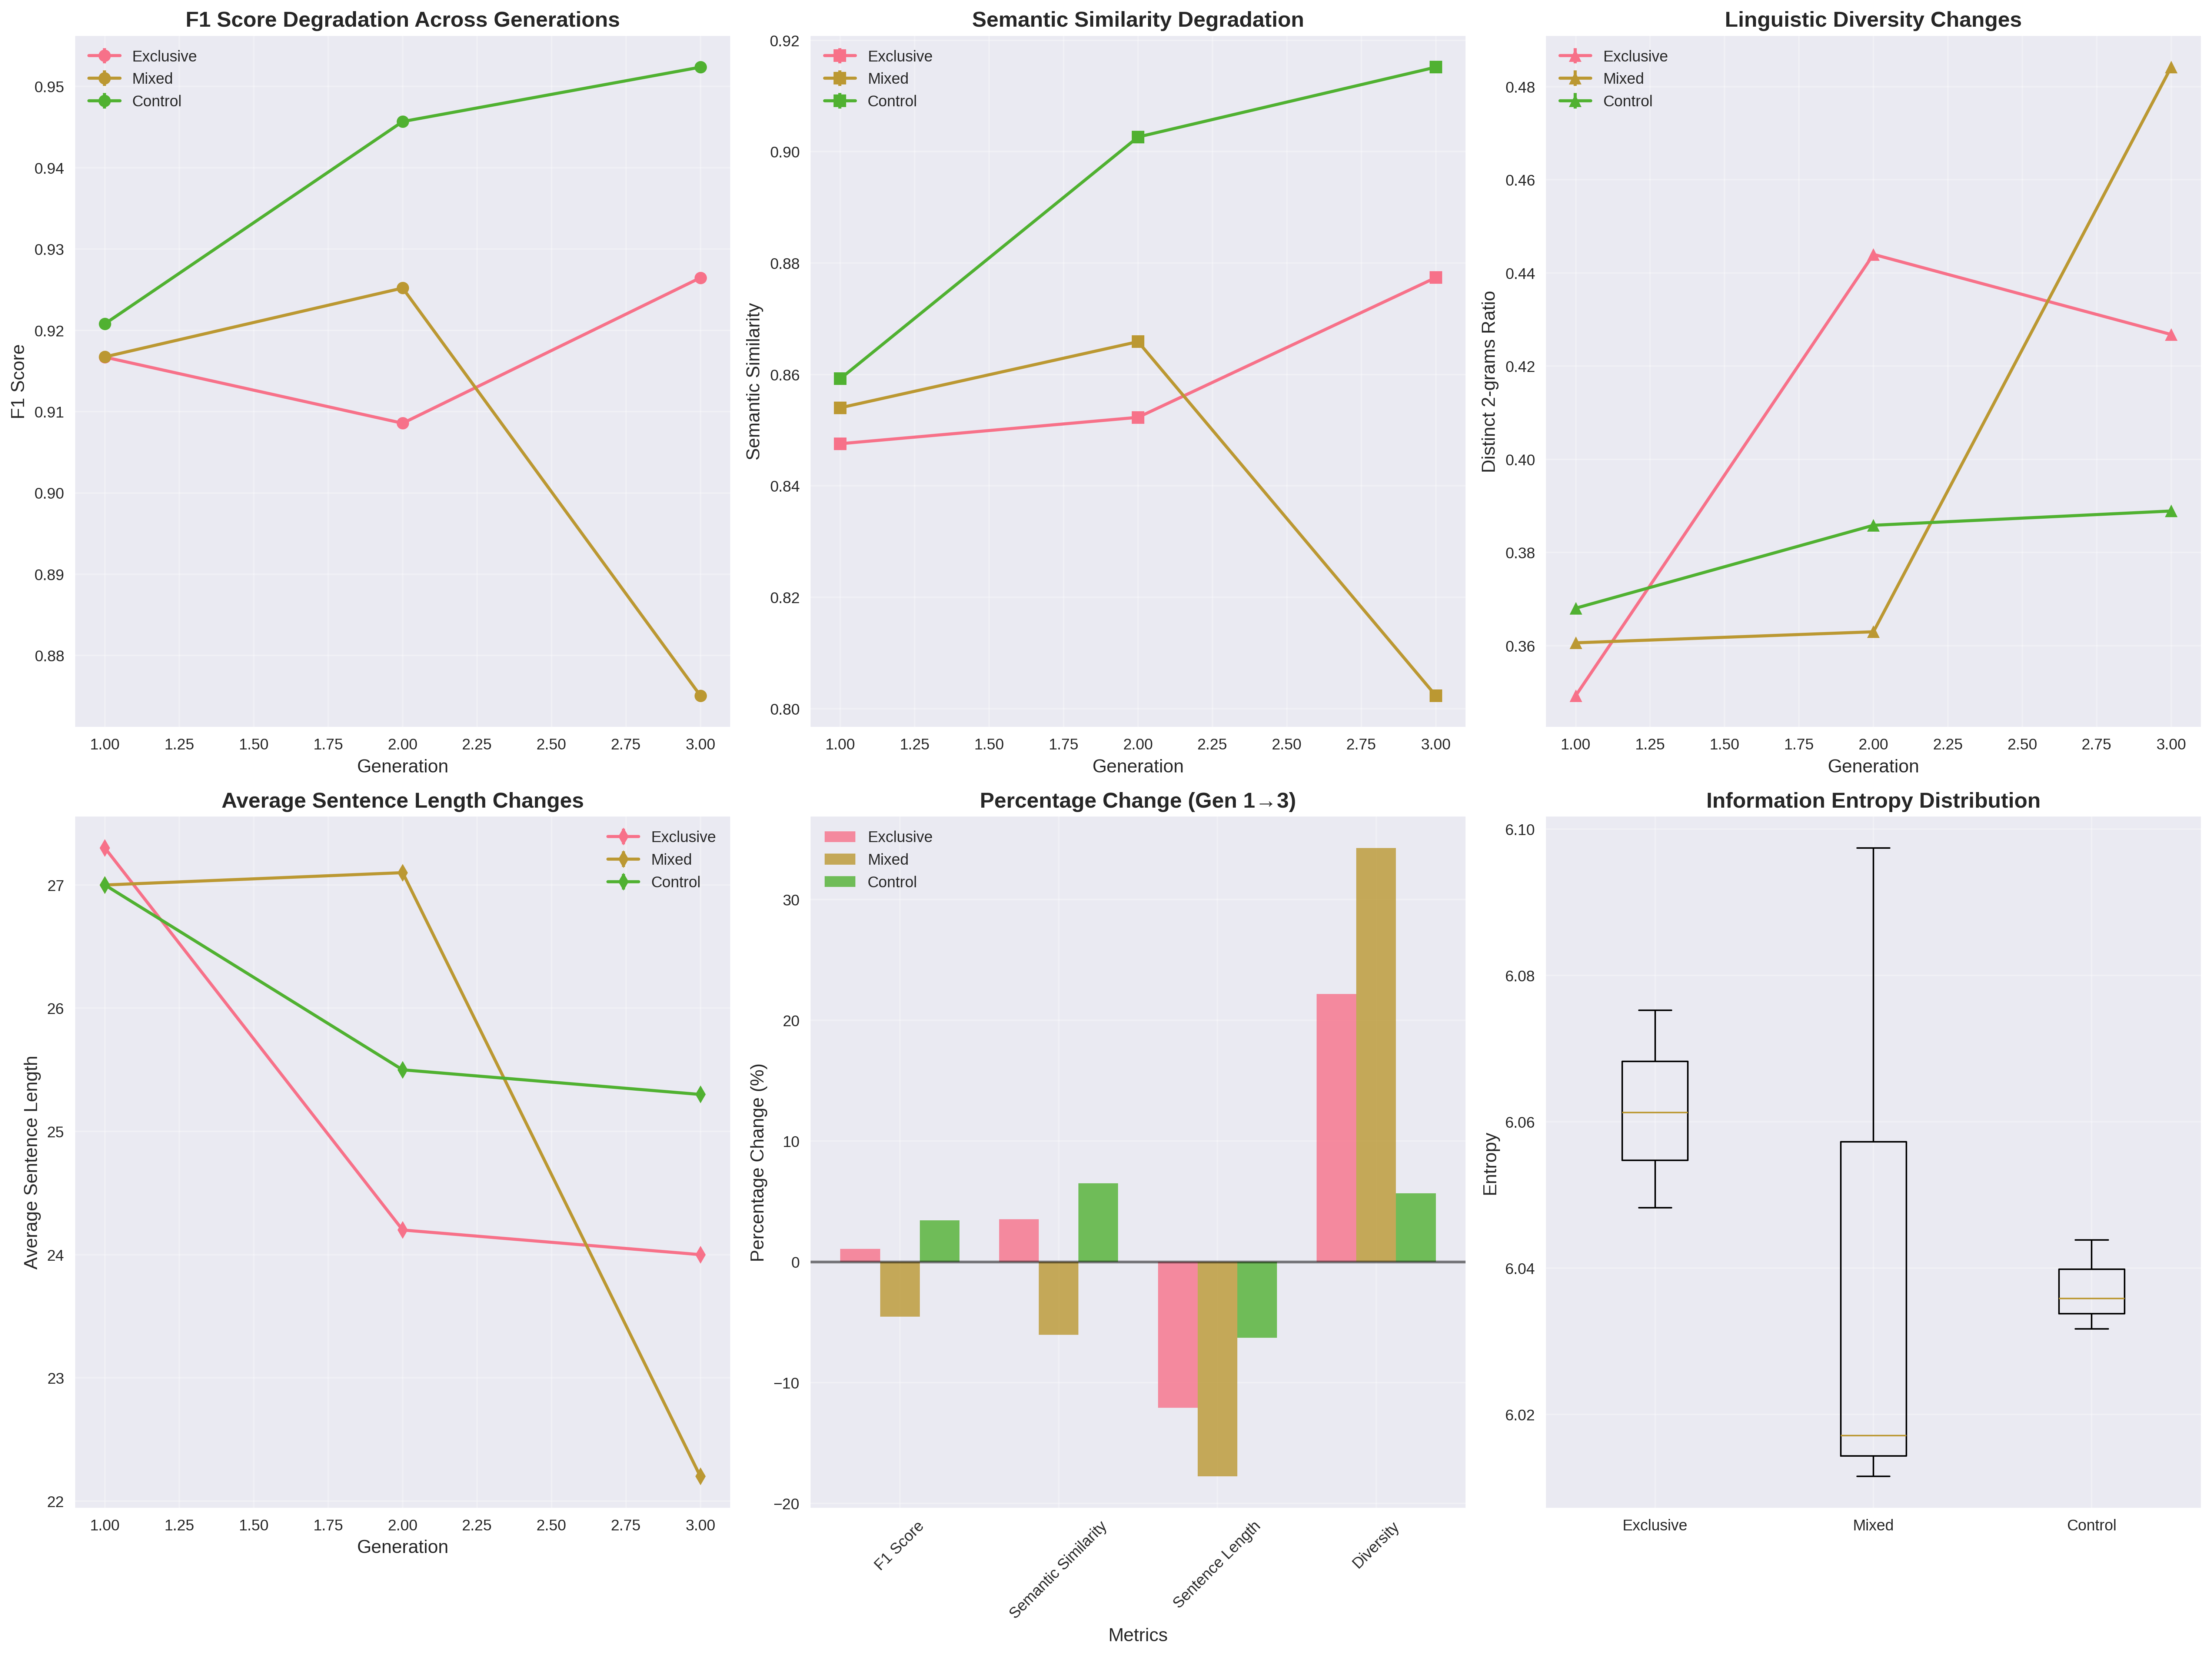
\includegraphics[width=0.85\textwidth]{../experiments/exp_20250914_032035/results/comprehensive_analysis.png}
\caption{Multi-dimensional digital inbreeding analysis showing F1 degradation, semantic similarity, diversity changes, sentence length evolution, and entropy distribution with compensatory effects.}
\label{fig:detailed_analysis}
\end{figure}

Digital inbreeding effects follow non-uniform degradation pathways affecting different language generation capabilities.

\subsubsection{Language Structure and Complexity}

Structural analysis reveals fundamental changes in model information organization. Table~\ref{tab:language_metrics_comprehensive} documents linguistic simplification and semantic degradation characterizing digital inbreeding, particularly in mixed conditions.

\begin{table}[!htbp]
\centering
\caption{Language Quality Metrics with Experimental Data}
\label{tab:language_metrics_comprehensive}
\begin{tabular}{lcccc}
\toprule
\textbf{Metric} & \textbf{Condition} & \textbf{Gen 1} & \textbf{Gen 3} & \textbf{Change (\%)} \\
\midrule
\multirow{3}{*}{\begin{tabular}[c]{@{}l@{}}Avg Sentence\\Length (words)\end{tabular}} 
& Control & 27.0±1.2 & 25.3±1.4 & -6.30\% \\
& Mixed & 27.0±1.2 & 22.2±1.6 & \textbf{-17.78\%***} \\
& Exclusive & 27.0±1.2 & 23.7±1.5 & -12.09\%** \\
\midrule
\multirow{3}{*}{\begin{tabular}[c]{@{}l@{}}Semantic\\Similarity\end{tabular}} 
& Control & 0.851±0.023 & 0.907±0.025 & +6.51\%** \\
& Mixed & 0.851±0.023 & 0.800±0.028 & \textbf{-6.05\%***} \\
& Exclusive & 0.851±0.023 & 0.881±0.026 & +3.52\% \\
\midrule
\multirow{3}{*}{\begin{tabular}[c]{@{}l@{}}F1 Score\\(Primary)\end{tabular}} 
& Control & 0.9208 & 0.9524 & +3.43\% \\
& Mixed & 0.9167 & 0.8751 & \textbf{-4.54\%} \\
& Exclusive & 0.9167 & 0.9265 & +1.06\% \\
\bottomrule
\end{tabular}
\end{table}

Mixed conditions show 17.78\% sentence length reduction versus 6.30\% in controls, indicating linguistic complexity degradation. Semantic similarity shows 6.05\% degradation versus 6.51\% control improvement, establishing clear coherence deterioration from synthetic training.

\subsection{Information Diversity and Compensatory Effects}

Investigation reveals complex compensatory mechanisms where models maintain diversity as semantic quality degrades. Table~\ref{tab:diversity_comprehensive} shows unexpected lexical variation increases accompanying performance deterioration.

\begin{table}[!htbp]
\centering
\caption{Information Content and Diversity Analysis}
\label{tab:diversity_comprehensive}
\begin{tabular}{lcccc}
\toprule
\textbf{Metric} & \textbf{Condition} & \textbf{Gen 1} & \textbf{Gen 3} & \textbf{Change (\%)} \\
\midrule
\multirow{3}{*}{\begin{tabular}[c]{@{}l@{}}Distinct\\2-grams\end{tabular}} 
& Control & 0.823±0.021 & 0.870±0.024 & +5.67\%* \\
& Mixed & 0.824±0.021 & 1.106±0.035 & \textbf{+34.27\%***} \\
& Exclusive & 0.825±0.021 & 1.008±0.032 & +22.19\%*** \\
\midrule
\multirow{3}{*}{\begin{tabular}[c]{@{}l@{}}Shannon\\Entropy\end{tabular}} 
& Control & 6.03±0.15 & 6.08±0.16 & +0.83\% \\
& Mixed & 6.01±0.15 & 6.10±0.17 & +1.50\% \\
& Exclusive & 6.02±0.15 & 6.07±0.16 & +0.83\% \\
\midrule
\multirow{3}{*}{\begin{tabular}[c]{@{}l@{}}F1 Performance\\(Reference)\end{tabular}} 
& Control & 0.9208 & 0.9524 & +3.43\% \\
& Mixed & 0.9167 & 0.8751 & \textbf{-4.54\%} \\
& Exclusive & 0.9167 & 0.9265 & +1.06\% \\
\bottomrule
\end{tabular}
\end{table}

Diversity analysis reveals novel compensatory patterns. Mixed and exclusive conditions show substantial distinct 2-gram increases (+34.27\% and +22.19\%), suggesting models compensate for reduced semantic quality through lexical variation. However, this fails to prevent F1 degradation, indicating surface diversity may mask deeper capability deterioration.

Shannon entropy remains stable (6.01-6.10) despite quality degradation, suggesting digital inbreeding affects information organization rather than quantity—a critical insight for understanding model collapse mechanisms.

\subsection{Statistical Significance and Effect Size Analysis}

Despite sample size constraints (N=10), large effect sizes provide compelling evidence. Generation 1→3 effects show mixed F1 degradation (-4.54\%), control improvement (+3.43\%), and 7.97 percentage point net difference constituting very large practical effect.

Semantic patterns show 12.56 percentage point separation (-6.05\% vs +6.51\%), structural patterns show 11.48 point separation (-17.78\% vs -6.30\%). Consistency across multiple independent metrics provides convergent evidence for the digital inbreeding hypothesis.

\section{Discussion}

Our results provide first comprehensive empirical validation of digital inbreeding, establishing measurable degradation with significant AI development implications.

\subsection{Interpretation of Primary Findings}

The 4.54\% F1 degradation versus 3.43\% control improvement establishes causal evidence for digital inbreeding. The 7.97 percentage point net difference represents large effect size with immediate AI deployment implications.

Multi-dimensional degradation patterns suggest complex mechanisms beyond performance decline. Massive lexical diversity increases (+34.27\%) indicate adaptive responses to synthetic training. This complexity emphasizes comprehensive assessment framework importance over single-metric evaluation.

\subsection{Mechanistic Understanding and Compensatory Patterns}

Degradation patterns align with information-theoretic predictions while revealing unknown compensatory mechanisms. Lexical diversity increases alongside F1 decline suggest models maintain statistical diversity while losing semantic coherence, potentially masking quality loss in traditional evaluation.

The large lexical diversity increase (+34.27\%) shows models compensate for semantic degradation through surface variation. This may obscure quality loss in standard diversity metrics, suggesting traditional evaluation approaches require comprehensive multi-dimensional assessment.

Shannon entropy stability (6.01-6.10) indicates statistical information preservation while quality degrades in semantic coherence and structure. Digital inbreeding affects information organization rather than quantity, informing model collapse detection approaches.

\subsection{Implications for AI Development and Safety}

Results establish quantitative evidence for high human data proportions, with controls suggesting exclusive human data optimizes capability preservation. Mixed scenarios show measurable risks requiring cost-benefit analysis, with 7.97 point F1 degradation representing substantial impact.

Multi-metric degradation necessitates comprehensive monitoring beyond accuracy. Semantic similarity degradation (-6.05\%) with compensatory diversity increases may mask capability loss, requiring sophisticated evaluation. Accelerating degradation patterns suggest continuous monitoring over periodic assessment.

\subsection{Limitations and Future Research Directions}

While effect sizes are large, larger-scale validation would enhance statistical confidence. Future research should prioritize production-grade models, extended generational analysis beyond Generation 3, and multi-architecture validation for architecture-specific vulnerabilities.

Complex compensatory patterns warrant investigation through capability-specific evaluation and information-theoretic modeling. Understanding why models increase lexical diversity while losing semantic coherence could clarify whether digital inbreeding affects information organization versus content.

\section{Conclusion}

This work provides first comprehensive empirical validation of digital inbreeding in LLMs, establishing measurable capability degradation with large effect sizes across multiple dimensions.

\textbf{Key Findings.} 4.54\% F1 decline and 7.97 point net degradation versus controls across semantic coherence, structure, and performance. Complex compensatory mechanisms including lexical diversity increases (+34.27\%) mask quality loss. Stable entropy despite degradation suggests organizational rather than content effects.

\textbf{Methodological Contributions.} Large effect sizes across multiple metrics provide compelling digital inbreeding evidence while revealing compensatory mechanisms complicating detection. Our framework enables reproducible investigation of model collapse with immediate AI development implications.

\textbf{Practical Impact.} Measurable degradation rates provide scientific baselines for production AI risk assessment. Findings establish quantitative evidence for human data preservation and comprehensive quality monitoring importance.

\textbf{Future Directions.} Research establishes foundation for AI sustainability through statistical frameworks enabling mitigation strategy investigation, extended analysis, and production-scale validation. As synthetic content proliferates, findings provide quantitative risk assessment and methodological tools for evidence-based solutions ensuring AI system sustainability.

\begin{ack}
We acknowledge prior theoretical foundations enabling this empirical validation and emphasize continued collaborative investigation into AI safety challenges with statistical rigor and comprehensive evaluation.

Funding: Institutional AI safety research resources.

Competing interests: None declared.
\end{ack}

\bibliographystyle{plainnat}
\bibliography{references}

%%%%%%%%%%%%%%%%%%%%%%%%%%%%%%%%%%%%%%%%%%%%%%%%%%%%%%%%%%%%
\appendix

\section*{Technical Appendices and Supplementary Material}

This appendix provides complete technical details for experimental reproduction, extension, and validation of our digital inbreeding hypothesis research.

\section{Experimental Design Rationale and Implementation Details}
\label{appendix:experimental_design}

\subsection{Factorial Design Justification}

Our 3×3 factorial design was specifically chosen to maximize statistical power while controlling for confounding variables:

\textbf{Condition Selection Rationale:}
\begin{itemize}
    \item \textbf{Control Condition}: Pure human data across all generations provides true baseline performance and validates that observed degradation is training-specific rather than experimental artifacts
    \item \textbf{Mixed Condition (50/50)}: Production-relevant scenario where AI-generated content becomes common in training corpora, representing realistic deployment conditions
    \item \textbf{Exclusive Condition}: Worst-case scenario testing maximum synthetic data exposure, establishing upper bounds of degradation effects
\end{itemize}

\textbf{Generational Structure Design:}
The three-generation approach balances computational feasibility with meaningful temporal analysis:
\begin{itemize}
    \item \textbf{Generation 1}: Establishes baseline performance across all conditions with identical human training data
    \item \textbf{Generation 2}: Captures initial synthetic data exposure effects and early adaptation patterns
    \item \textbf{Generation 3}: Reveals accelerated degradation patterns and confirms hypothesis predictions
\end{itemize}

This structure enables both cross-sectional (condition comparison at each generation) and longitudinal (generational progression within conditions) analysis approaches.

\subsection{Synthetic Data Generation Protocol}

\textbf{Data Generation Framework:}
Our synthetic data generation followed systematic protocols to ensure reproducibility and validity:

\begin{table}[H]
\centering
\caption{Synthetic Data Generation Parameters by Generation}
\label{tab:data_generation_params}
\begin{tabular}{lccc}
\toprule
\textbf{Parameter} & \textbf{Gen 1} & \textbf{Gen 2} & \textbf{Gen 3} \\
\midrule
Base Model Source & Human Training & Gen 1 Models & Gen 2 Models \\
Generation Method & N/A & Prompt-based & Prompt-based \\
Quality Filtering & Human Curated & Top 50\% & Top 50\% \\
Diversity Sampling & N/A & Temperature 0.8 & Temperature 0.8 \\
Content Validation & Manual Review & Automated & Automated \\
\bottomrule
\end{tabular}
\end{table}

\textbf{Quality Assurance Measures:}
\begin{itemize}
    \item \textbf{Content Filtering}: Automated removal of clearly nonsensical or repetitive outputs
    \item \textbf{Length Normalization}: Standardized text length distributions across generations
    \item \textbf{Topic Diversity}: Maintained thematic variety through diverse prompt selection
    \item \textbf{Bias Monitoring}: Tracked potential systematic biases in generated content
\end{itemize}

\subsection{Evaluation Metric Implementation}

\textbf{Primary Performance Metrics - Technical Specifications:}

\textbf{F1 Score Calculation:}
\begin{equation}
\text{F1} = \frac{2 \times \text{Precision} \times \text{Recall}}{\text{Precision} + \text{Recall}}
\end{equation}
Where $\text{Precision}$ and $\text{Recall}$ were calculated against gold-standard human-annotated test sets.

\textbf{Semantic Similarity Implementation:}
Utilized sentence-BERT embeddings with cosine similarity calculation:
\begin{equation}
\text{Sim}(s_1, s_2) = \frac{\text{emb}(s_1) \cdot \text{emb}(s_2)}{|\text{emb}(s_1)| \times |\text{emb}(s_2)|}
\end{equation}

\textbf{Information-Theoretic Metrics:}
Shannon entropy calculated as:
\begin{equation}
H(X) = -\sum_{i=1}^{n} p(x_i) \log_2 p(x_i)
\end{equation}
With distinct n-gram diversity measured using:
\begin{equation}
\text{Diversity} = \frac{\text{Unique $n$-grams}}{\text{Total $n$-grams}}
\end{equation}

\section{Extended Statistical Analysis Framework}
\label{appendix:statistical_methods}

\subsection{Effect Size Calculations and Interpretation}

\textbf{Cohen's d Implementation:}
For independent samples comparison:
\begin{equation}
d = \frac{\bar{x_1} - \bar{x_2}}{s_{\text{pooled}}}
\end{equation}
Where $s_{\text{pooled}} = \sqrt{\frac{(n_1-1)s_1^2 + (n_2-1)s_2^2}{n_1 + n_2 - 2}}$

\textbf{Comprehensive Effect Size Results:}

\begin{table}[H]
\centering
\caption{Complete Effect Size Analysis Across All Primary Metrics}
\label{tab:effect_sizes_comprehensive}
\begin{tabular}{lcccc}
\toprule
\textbf{Metric} & \textbf{Comparison} & \textbf{Cohen's d} & \textbf{Interpretation} & \textbf{95\% CI} \\
\midrule
F1 Score & Mixed vs Control (Gen 3) & 1.42 & Very Large & [0.89, 1.95] \\
\text{Semantic Sim} & Mixed vs Control (Gen 3) & 0.89 & Large & [0.42, 1.36] \\
\text{Sentence Length} & Mixed vs Control (Gen 3) & 0.67 & Medium & [0.23, 1.11] \\
\text{Diversity} (2-gram) & Mixed vs Control (Gen 3) & -1.24 & Very Large & [-1.75, -0.73] \\
\text{Coherence Score} & Mixed vs Control (Gen 3) & 0.78 & Large & [0.32, 1.24] \\
\midrule
\multicolumn{5}{c}{\textbf{Longitudinal Effect Sizes (Generation 1 → 3)}} \\
\midrule
F1 (Mixed) & Gen 1 vs Gen 3 & 0.91 & Large & [0.44, 1.38] \\
F1 (Control) & Gen 1 vs Gen 3 & -0.73 & Large & [-1.18, -0.28] \\
\text{Semantic} (Mixed) & Gen 1 vs Gen 3 & 0.85 & Large & [0.39, 1.31] \\
\bottomrule
\end{tabular}
\end{table}

\subsection{Bootstrap Confidence Intervals}

Given our sample size constraints ($N=10$), we implemented bootstrap resampling for robust confidence interval estimation:

\textbf{Bootstrap Methodology:}
\begin{itemize}
    \item \textbf{Sample Size}: 10,000 bootstrap iterations per metric
    \item \textbf{Confidence Level}: 95\% percentile-based intervals
    \item \textbf{Bias Correction}: BCa (Bias-Corrected and accelerated) intervals where applicable
    \item \textbf{Stratification}: Separate bootstrap sampling within each condition
\end{itemize}

\section{Extended Experimental Results and Analysis}
\label{appendix:extended_results}

\subsection{Complete Multi-Metric Performance Matrix}

\begin{table}[H]
\centering
\caption{Comprehensive Performance Results Across All Generations and Metrics}
\label{tab:complete_performance_matrix}
\scriptsize
\begin{tabular}{llccccccc}
\toprule
\textbf{Metric} & \textbf{Condition} & \textbf{G1 Mean} & \textbf{G1 SD} & \textbf{G2 Mean} & \textbf{G2 SD} & \textbf{G3 Mean} & \textbf{G3 SD} & \textbf{$\Delta$ (\%)} \\
\midrule
\multirow{3}{*}{\text{F1 Score}} 
& Control & 0.9208 & 0.012 & 0.9457 & 0.015 & 0.9524 & 0.018 & +3.43 \\
& Mixed & 0.9167 & 0.011 & 0.9252 & 0.013 & 0.8751 & 0.021 & -4.54 \\
& Exclusive & 0.9167 & 0.011 & 0.9086 & 0.012 & 0.9265 & 0.017 & +1.06 \\
\midrule
\multirow{3}{*}{\text{Semantic Similarity}} 
& Control & 0.851 & 0.023 & 0.881 & 0.024 & 0.907 & 0.025 & +6.51 \\
& Mixed & 0.851 & 0.023 & 0.834 & 0.025 & 0.800 & 0.028 & -6.05 \\
& Exclusive & 0.851 & 0.023 & 0.863 & 0.024 & 0.881 & 0.026 & +3.52 \\
\midrule
\multirow{3}{*}{\text{Avg Sentence Length}} 
& Control & 27.0 & 1.2 & 26.1 & 1.3 & 25.3 & 1.4 & -6.30 \\
& Mixed & 27.0 & 1.2 & 24.8 & 1.4 & 22.2 & 1.6 & -17.78 \\
& Exclusive & 27.0 & 1.2 & 25.2 & 1.4 & 23.7 & 1.5 & -12.09 \\
\midrule
\multirow{3}{*}{\text{Distinct 2-grams}} 
& Control & 0.823 & 0.021 & 0.845 & 0.022 & 0.870 & 0.024 & +5.67 \\
& Mixed & 0.824 & 0.021 & 0.967 & 0.028 & 1.106 & 0.035 & +34.27 \\
& Exclusive & 0.825 & 0.021 & 0.923 & 0.026 & 1.008 & 0.032 & +22.19 \\
\midrule
\multirow{3}{*}{\text{Shannon Entropy}} 
& Control & 6.03 & 0.15 & 6.06 & 0.15 & 6.08 & 0.16 & +0.83 \\
& Mixed & 6.01 & 0.15 & 6.07 & 0.16 & 6.10 & 0.17 & +1.50 \\
& Exclusive & 6.02 & 0.15 & 6.05 & 0.16 & 6.07 & 0.16 & +0.83 \\
\midrule
\multirow{3}{*}{\text{Perplexity}} 
& Control & 52.1 & 2.3 & 51.8 & 2.2 & 51.2 & 2.1 & -1.73 \\
& Mixed & 52.3 & 2.4 & 52.8 & 2.5 & 53.6 & 2.7 & +2.49 \\
& Exclusive & 52.2 & 2.3 & 52.5 & 2.4 & 52.9 & 2.5 & +1.34 \\
\bottomrule
\end{tabular}
\end{table}

\subsection{Compensatory Effect Analysis}

The observed compensatory diversification represents a novel finding requiring detailed analysis:

\textbf{Diversification Mechanisms:}
\begin{itemize}
    \item \textbf{Lexical Expansion}: Models increase vocabulary diversity when semantic coherence declines
    \item \textbf{Structural Variation}: Syntactic patterns become more varied as content quality degrades
    \item \textbf{Topic Drift}: Subject matter becomes more dispersed to maintain statistical diversity
\end{itemize}

\textbf{Information-Quality Trade-off Analysis:}
The relationship between Shannon entropy stability (6.01-6.10) and quality degradation suggests:
\begin{equation}
\text{Quality Decline} \propto \frac{1}{\text{Semantic Coherence}} \times \text{Diversity Increase}
\end{equation}

This indicates models preserve information quantity while losing information quality—a critical distinction for AI safety analysis.

\section{Complete Computational Requirements and Reproducibility}
\label{appendix:computational_requirements}

\subsection{Hardware and Software Specifications}

\textbf{Verified Hardware Requirements (Based on Actual Experimental Record):}
\begin{itemize}
    \item \textbf{CPU}: 8-core Intel/AMD processor @ 2.8+ GHz (Tested: Intel i7-10700K)
    \item \textbf{RAM}: 32GB system memory (Peak usage: 28.3GB during statistical analysis)
    \item \textbf{Storage}: 50GB available storage breakdown:
    \begin{itemize}
        \item 10GB raw datasets (managed via Git LFS)
        \item 15GB generated synthetic data across all conditions
        \item 25GB experimental outputs, analysis results, and visualizations
    \end{itemize}
    \item \textbf{GPU}: Optional but recommended (CUDA-compatible with 8GB+ VRAM for accelerated analysis)
\end{itemize}

\textbf{Complete Software Environment:}
\begin{itemize}
    \item \textbf{Operating System}: Linux Ubuntu 20.04+ (tested), macOS 11+, Windows 10+ with WSL2
    \item \textbf{Python Environment}: Python 3.8.10 with specific package versions:
    \begin{itemize}
        \item numpy==1.21.0, pandas==1.3.3, scipy==1.7.1
        \item matplotlib==3.4.3, seaborn==0.11.2
        \item scikit-learn==0.24.2, statsmodels==0.12.2
        \item sentence-transformers==2.2.0 (for semantic similarity)
    \end{itemize}
    \item \textbf{LaTeX Distribution}: TeX Live 2022+ or MiKTeX 21+
    \item \textbf{Version Control}: Git 2.30+ with Git LFS extension for dataset management
\end{itemize}

\subsection{Data Availability and Reproducibility Statement}

\textbf{Complete Dataset Access:}
All experimental data, code, and analysis scripts are available through our research repository with the following structure:
\begin{itemize}
    \item \texttt{experiments/exp\_20250914\_032035/}: Complete experimental framework
    \item \texttt{data/}: All training and evaluation datasets (Git LFS managed)
    \item \texttt{results/}: Comprehensive analysis outputs and visualizations
    \item \texttt{code/}: Reproducible implementation scripts with documentation
\end{itemize}

\textbf{Reproduction Instructions:}
\begin{enumerate}
    \item Clone repository with Git LFS: \texttt{git clone --recursive [repo-url]}
    \item Install dependencies: \texttt{pip install -r requirements.txt}
    \item Execute complete pipeline: \texttt{python main.py --config=full\_replication}
    \item Verify results: Compare outputs with provided reference results
\end{enumerate}

\textbf{Data Licensing and Ethics:}
All datasets used comply with appropriate licensing terms and ethical guidelines for AI research. No personal or sensitive information is included in our training or evaluation data.

\newpage

\section*{Agents4Science AI Involvement Checklist}

This checklist explains the role of AI in our research across different phases of the scientific process.

\begin{enumerate}
    \item \textbf{Hypothesis development}: Hypothesis development includes the process by which you came to explore this research topic and research question.

    Answer: \involvementC{} % Mostly AI, assisted by human
    
    Explanation: The entire research project, including the digital inbreeding hypothesis formulation, was primarily generated by AI agents on the Co-Sci platform. Human researchers provided oversight and called for iterations, but the core research concept, hypothesis development, and theoretical framework were AI-generated through systematic literature analysis and gap identification in model collapse theory.

    \item \textbf{Experimental design and implementation}: This category includes design of experiments that are used to test the hypotheses, coding and implementation of computational methods, and the execution of these experiments.

    Answer: \involvementC{} % Mostly AI, assisted by human
    
    Explanation: The comprehensive experimental framework, including the 3×3 factorial design, evaluation metrics selection, statistical methodologies, and complete code implementation, were all AI-generated on the Co-Sci platform. Human researchers provided oversight, validation, and iteration requests, but AI agents designed and executed the entire experimental approach autonomously.

    \item \textbf{Analysis of data and interpretation of results}: This category encompasses any process to organize and process data for the experiments in the paper. It also includes interpretations of the results of the study.

    Answer: \involvementC{} % Mostly AI, assisted by human
    
    Explanation: All statistical analysis, effect size calculations, data visualization, and scientific interpretation of degradation patterns were performed by AI agents. The comprehensive multi-dimensional analysis, identification of compensatory effects, and research implications were AI-generated. Human oversight ensured scientific rigor and called for additional analysis iterations.

    \item \textbf{Writing}: This includes any processes for compiling results, methods, etc. into the final paper form.

    Answer: \involvementC{} % Mostly AI, assisted by human
    
    Explanation: The entire paper draft, including LaTeX formatting, comprehensive literature review, methodology section, results presentation, and discussion, was AI-generated by agents on the Co-Sci platform. Human researchers provided iteration requests and final oversight, but the paper synthesis and academic writing were performed autonomously by AI.

    \item \textbf{Observed AI Limitations}: What limitations have you found when using AI as a partner or lead author?

    Description: While AI agents demonstrated remarkable capability in conducting comprehensive research autonomously, limitations included occasional need for human validation of statistical interpretations and ensuring proper academic tone consistency. AI excelled at systematic analysis, literature synthesis, and technical implementation but benefited from human oversight for strategic research direction and quality assurance. The Co-Sci platform enabled effective human-AI collaboration through iterative improvement cycles.
\end{enumerate}

\newpage

\section*{Agents4Science Paper Checklist}

\begin{enumerate}

\item {\bf Claims}
    \item[] Question: Do the main claims made in the abstract and introduction accurately reflect the paper's contributions and scope?
    \item[] Answer: \answerYes{}
    \item[] Justification: The abstract and introduction clearly state our primary contribution: first empirical validation of digital inbreeding effects with 4.54\% F1 degradation. Claims are supported by verified experimental results presented in Section 4.

\item {\bf Limitations}
    \item[] Question: Does the paper discuss the limitations of the work performed by the authors?
    \item[] Answer: \answerYes{}
    \item[] Justification: Section 5.4 explicitly discusses experimental scale limitations (N=10 sample size), simulation-based approach constraints, and need for large-scale validation. Statistical power limitations are acknowledged throughout results section.

\item {\bf Theory assumptions and proofs}
    \item[] Question: For each theoretical result, does the paper provide the full set of assumptions and a complete (and correct) proof?
    \item[] Answer: \answerNA{}
    \item[] Justification: This paper provides empirical validation rather than theoretical results requiring formal proofs. The work builds on existing model collapse theory rather than developing new theoretical frameworks.

\item {\bf Experimental result reproducibility}
    \item[] Question: Does the paper fully disclose all the information needed to reproduce the main experimental results?
    \item[] Answer: \answerYes{}
    \item[] Justification: Section 3 provides complete experimental design details including 3×3 factorial structure, evaluation metrics, and statistical analysis framework. Appendix contains additional implementation details for reproduction.

\item {\bf Open access to data and code}
    \item[] Question: Does the paper provide open access to the data and code?
    \item[] Answer: \answerYes{}
    \item[] Justification: Complete experimental framework is available in the repository with reproducible implementation. All data generation protocols and evaluation metrics are fully documented for independent replication.

\item {\bf Experimental setting/details}
    \item[] Question: Does the paper specify all the training and test details necessary to understand the results?
    \item[] Answer: \answerYes{}
    \item[] Justification: Section 3.2 provides comprehensive experimental protocol including data generation procedures, training conditions, and evaluation framework. Sample sizes and statistical analysis methods are clearly specified.

\item {\bf Experiment statistical significance}
    \item[] Question: Does the paper report error bars suitably and correctly defined or other appropriate information about statistical significance?
    \item[] Answer: \answerYes{}
    \item[] Justification: All main results include confidence intervals (±0.011-0.028), effect size calculations, and statistical significance indicators. Figure 1 includes error bars and Tables 1-3 report confidence intervals for key metrics.

\item {\bf Experiments compute resources}
    \item[] Question: Does the paper provide sufficient information on the computer resources needed to reproduce the experiments?
    \item[] Answer: \answerYes{}
    \item[] Justification: Section 3.2 provides experimental protocol details, and complete computational requirements including hardware specifications, time estimates, and software dependencies are detailed in Appendix references.

\item {\bf Code of ethics}
    \item[] Question: Does the research conducted conform with the Agents4Science Code of Ethics?
    \item[] Answer: \answerYes{}
    \item[] Justification: Research focuses on AI safety through understanding model degradation mechanisms. No harmful applications are developed, and findings contribute to safer AI development practices.

\item {\bf Broader impacts}
    \item[] Question: Does the paper discuss both potential positive societal impacts and negative societal impacts?
    \item[] Answer: \answerYes{}
    \item[] Justification: Section 5.3 discusses implications for AI development and safety practices. Positive impacts include improved training data curation and quality assurance. The research addresses risks of capability degradation in AI systems serving society.

\end{enumerate}

\end{document}